\documentclass[10pt,a4paper]{article}
\usepackage[utf8]{inputenc}
\usepackage{amsmath}
\usepackage{amsfonts}
\usepackage{amssymb}
\usepackage{fullpage}
\usepackage{booktabs}
\usepackage{caption}
\usepackage{subcaption}
\usepackage{graphicx}
\usepackage{epstopdf} 

\author{Christoph Aymanns}
\begin{document}
\section{Definitions}
Let:
\begin{itemize}
\item Adjacency matrix of network: $\mathbf{A}$
\item Neighbourhood of a given node: $B$ 
\item Size of neighbourhood: $k =|B|$: 
\item Number of node in network: $n$.
\item Action vector: $\mathbf{x}$.
\item Private belief: $p$ 
\item Social belief: $q = \sum_{i \in B} x_i / k = \mathbf{A} \mathbf{x} / k$. 
\item Threshold function: $f(p,q)$ such that:
\begin{equation}
x = \begin{cases} 1 &\mbox{if } f(p,q) > 0.5  \\
0 & \mbox{if } f(p,q) < 0.5 \end{cases}
\end{equation}
\end{itemize}
We distinguish between three cases for the threshold function:
\begin{enumerate}
\item ``Equal'':
\begin{equation}
f(p,q) = 0.5(p+q).
\end{equation}
\item ``Neighbor'':
\begin{equation}
f(p,q) = \frac{1}{k+1}p + \frac{k}{k+1}q.
\end{equation}
\item ``Rel Neighbor'':
\begin{equation}
f(p,q) = \left(1 - \frac{k}{n-1}\right) p + \frac{k}{n-1}q.
\end{equation}
\end{enumerate}

\section{Figures for exogenous network case}

\begin{table}[h]
\begin{tabular}{llrrr} 
\toprule
Notation & Description & Value \\
\cmidrule{3-5}
&  & 1 - (I) & 2 - (U) & 3 - (U) \\
\midrule
$N$ & Number of agents & $100$ & $100$ & $100$ \\ 
$\mu_0$ & Average signal for $\theta = 0$ & $0.4$ & $0.49$ & $0.3$ \\ 
$\mu_1$ & Average signal for $\theta = 1$ & $0.6$ & $0.51$ & $0.7$ \\ 
$\sigma_0$ & Standard deviation of signal for $\theta = 0$ & $\sqrt{0.1}$ & $\sqrt{0.1}$ & $\sqrt{0.1}$ \\ 
$\sigma_1$ & Standard deviation of signal for $\theta = 1$ & $\sqrt{0.1}$ & $\sqrt{0.1}$ & $\sqrt{0.1}$ \\ 
$T$ & Number of iterations of updater & $100$ & $100$ & $100$ \\ 
$\rho$ & Density of ER network & $[0,0.95]$ & $[0,0.95]$ & $0.5$ \\ 
$p$ & Probability of being informed & NA & NA & $[0.1,0.9]$ \\ 
$S$ & Number of simulations per parameter configuration & $1000$ & $1000$ & $1000$ \\ 
\bottomrule 
\end{tabular}
\caption{Parameters for runs for the three cases above.}
\end{table}

Throughout this document we assume that the state of the world is $\theta = 1$.
We consider three cases below:
\begin{enumerate}
\item Informed agents (I): a population of 100 agents connected via an ER network and a signal $\mu_0 = 0.4$
\item Uninformed agents (U): a population of 100 agents connected via an ER network and a signal $\mu_0 = 0.49$
\item Heterogeneous agents (H): a population of 100 agents connected via an ER network. With probability $p$ agents are either informed ($\mu_0 = 0.3$) or uninformed ($\mu_0 = 0.49$).
\end{enumerate}

Cases 1 and 2 we further sub-divide into the three cases for the threshold function (``equal'',``neighbor'',``rel neighbor'').

\clearpage

% =====================================
%
% CASE 1 - (I) - EQUAL
%
% =====================================

\begin{figure}[ht]
\centering
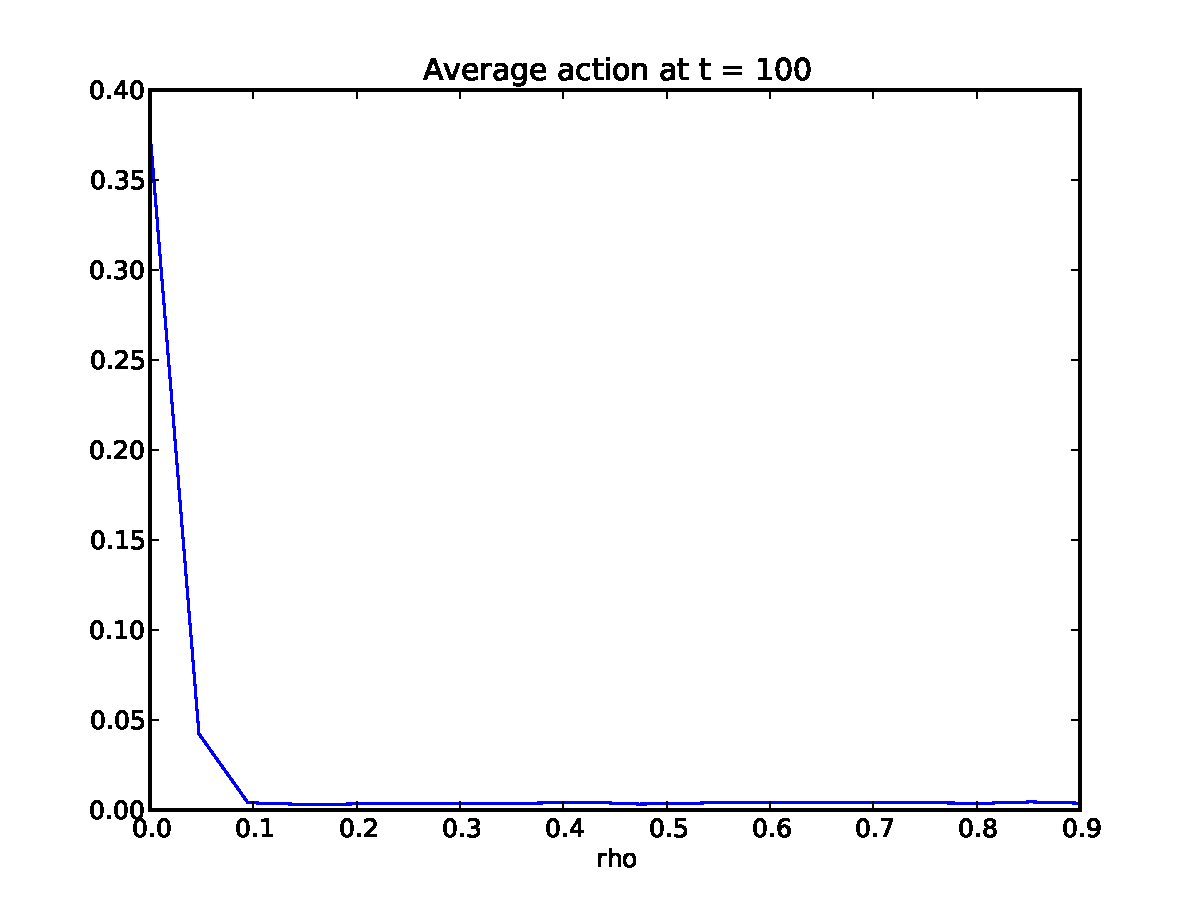
\includegraphics[width=0.5\textwidth]{figures/inf/EQUAL_N100_04_AVA}
\caption{Case 1 - (I) - equal: Average final action of agents as a function of the density of the ER network (rho). The average final action is defined as: $x_F = \sum_j x_j(T)/N$. Data shown is averaged over $S$ (1000) simulations per network density $\rho$. For $\rho = 0$ the agents' actions do not synchronize as they are solely determined by their private belief. As the network density is increased social learning leads to action synchronization.}
\end{figure}

\begin{figure}[ht]
\centering
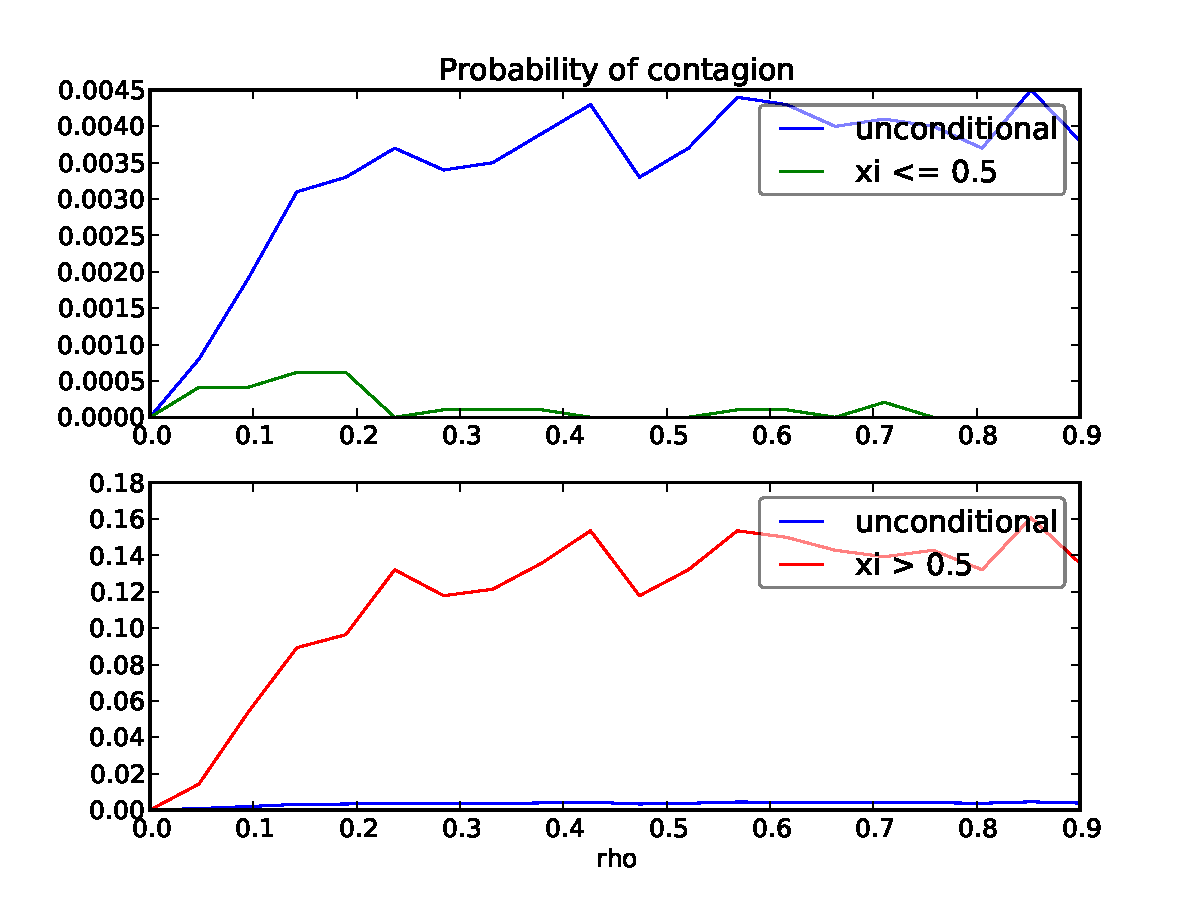
\includegraphics[width=0.5\textwidth]{figures/inf/EQUAL_N100_04_CONT}
\caption{Case 1 - (I) - equal : Fraction of simulations per parameter configuration $S$ (1000) in which agents synchronize on the state non matching action (more than 80\% of agents choose state non-matching action) as a function of network density (rho). We distinguish three cases: (1) unconditional: we compute the fraction based on the full sample $S$. (2) conditional $xi \leq 0.5$: we compute the fraction based on the sub-set of simulations in which the average initial action $x_i = \sum_j x_j(0)/N \leq 0.5$, i.e. when the agents start with a state matching action. (3) conditional $xi > 0.5$: we compute the fraction based on the sub-set of simulations in which the average initial action $x_i = \sum_j x_j(0)/N > 0.5$, i.e. when the agents start with a state non matching action.  }
\end{figure}

\begin{figure}[ht]
\centering
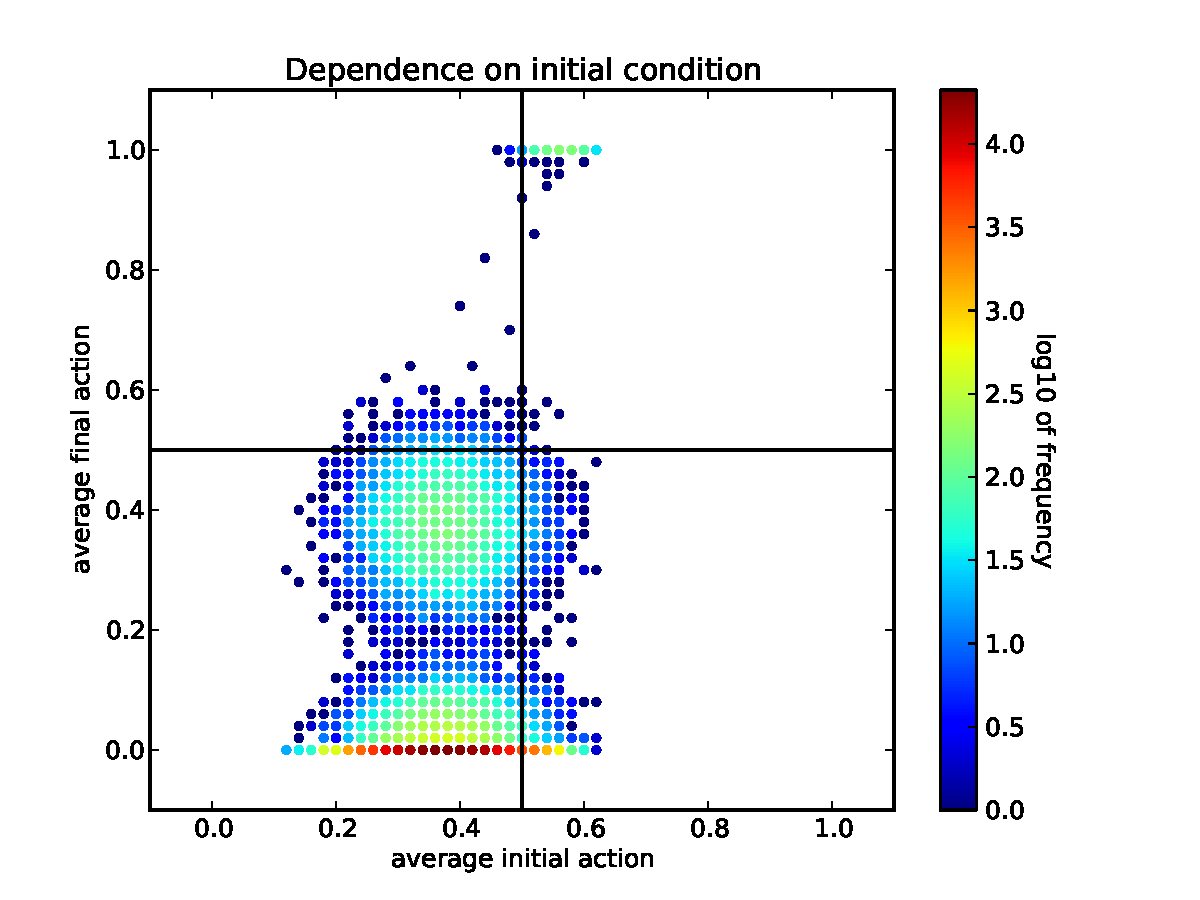
\includegraphics[width=0.5\textwidth]{figures/inf/EQUAL_N100_04_SCAT_HIST}
\caption{Case 1 - (I) - equal: We plot the average initial action $x_i = \sum_j x_j(0)/N$ vs. the average final action $x_F = \sum_j x_j(T)/N$. Data points are averages over $S$ (1000) simulations and all network densities $\rho$ (20 values equally distributed over the interval $[0,0.95]$. The color code indicates the frequency with which a point occurs in the sample (total size $20 \times 1000$), the scale of the color code is logarithmic of base 10.}
\end{figure}

% =====================================
%
% CASE 1 - (I) - NEIGHBOR
%
% =====================================

\begin{figure}[ht]
\centering
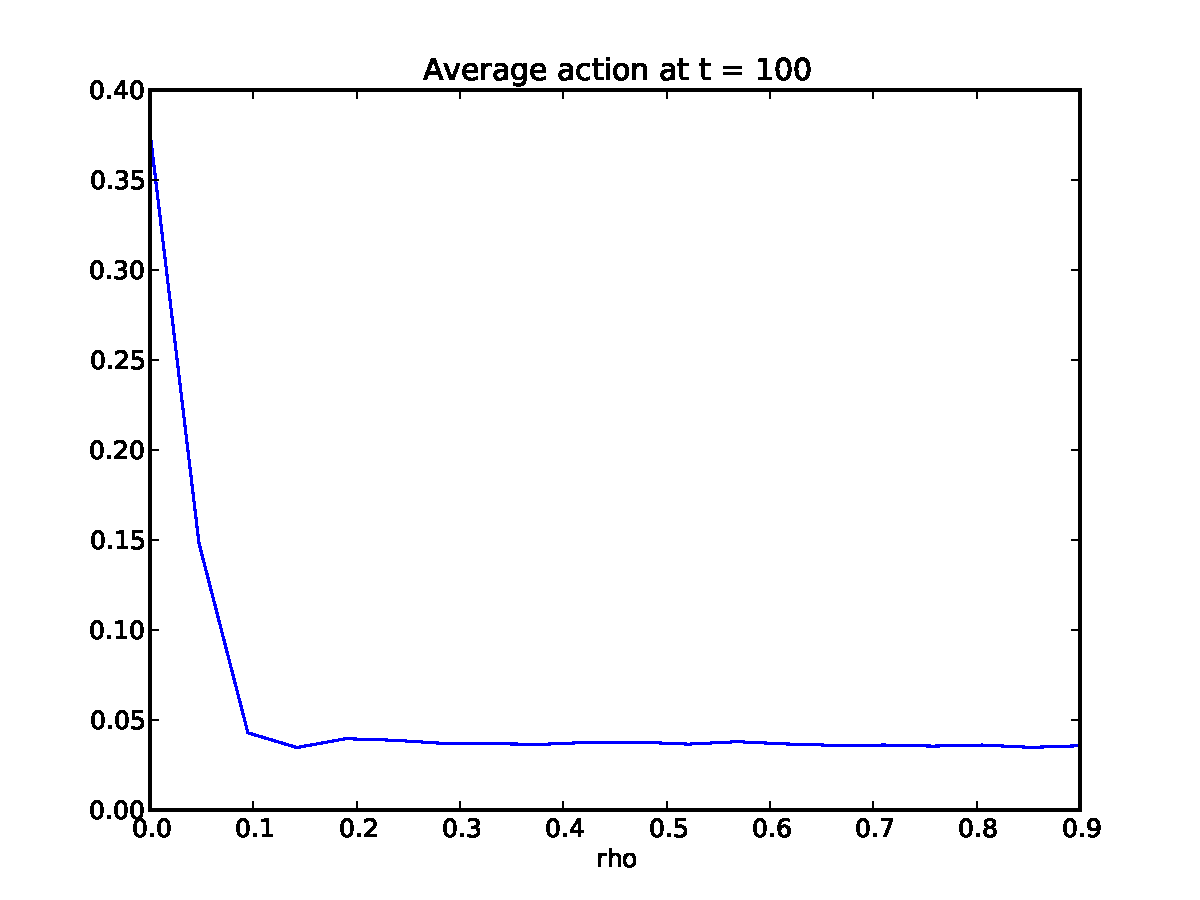
\includegraphics[width=0.5\textwidth]{figures/inf/NEIG_N100_04_AVA}
\caption{Case 1 - (I) - neighbor: Average final action of agents as a function of the density of the ER network (rho). The average final action is defined as: $x_F = \sum_j x_j(T)/N$. Data shown is averaged over $S$ (1000) simulations per network density $\rho$. For $\rho = 0$ the agents' actions do not synchronize as they are solely determined by their private belief. As the network density is increased social learning leads to action synchronization.}
\end{figure}

\begin{figure}[ht]
\centering
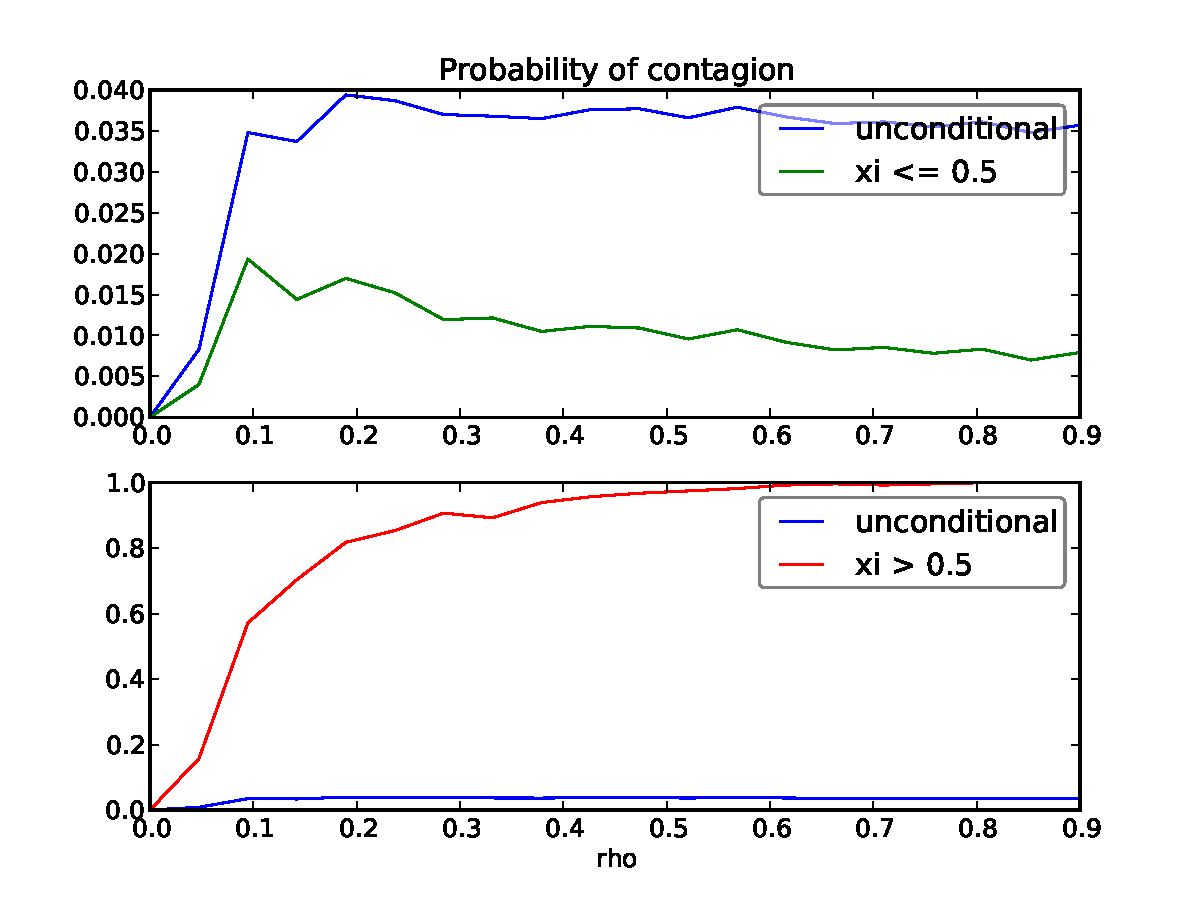
\includegraphics[width=0.5\textwidth]{figures/inf/NEIG_N100_04_CONT}
\caption{Case 1 - (I) - neighbor: Fraction of simulations per parameter configuration $S$ (1000) in which agents synchronize on the state non matching action (more than 80\% of agents choose state non-matching action) as a function of network density (rho). We distinguish three cases: (1) unconditional: we compute the fraction based on the full sample $S$. (2) conditional $xi \leq 0.5$: we compute the fraction based on the sub-set of simulations in which the average initial action $x_i = \sum_j x_j(0)/N \leq 0.5$, i.e. when the agents start with a state matching action. (3) conditional $xi > 0.5$: we compute the fraction based on the sub-set of simulations in which the average initial action $x_i = \sum_j x_j(0)/N > 0.5$, i.e. when the agents start with a state non matching action.  }
\end{figure}

\begin{figure}[ht]
\centering
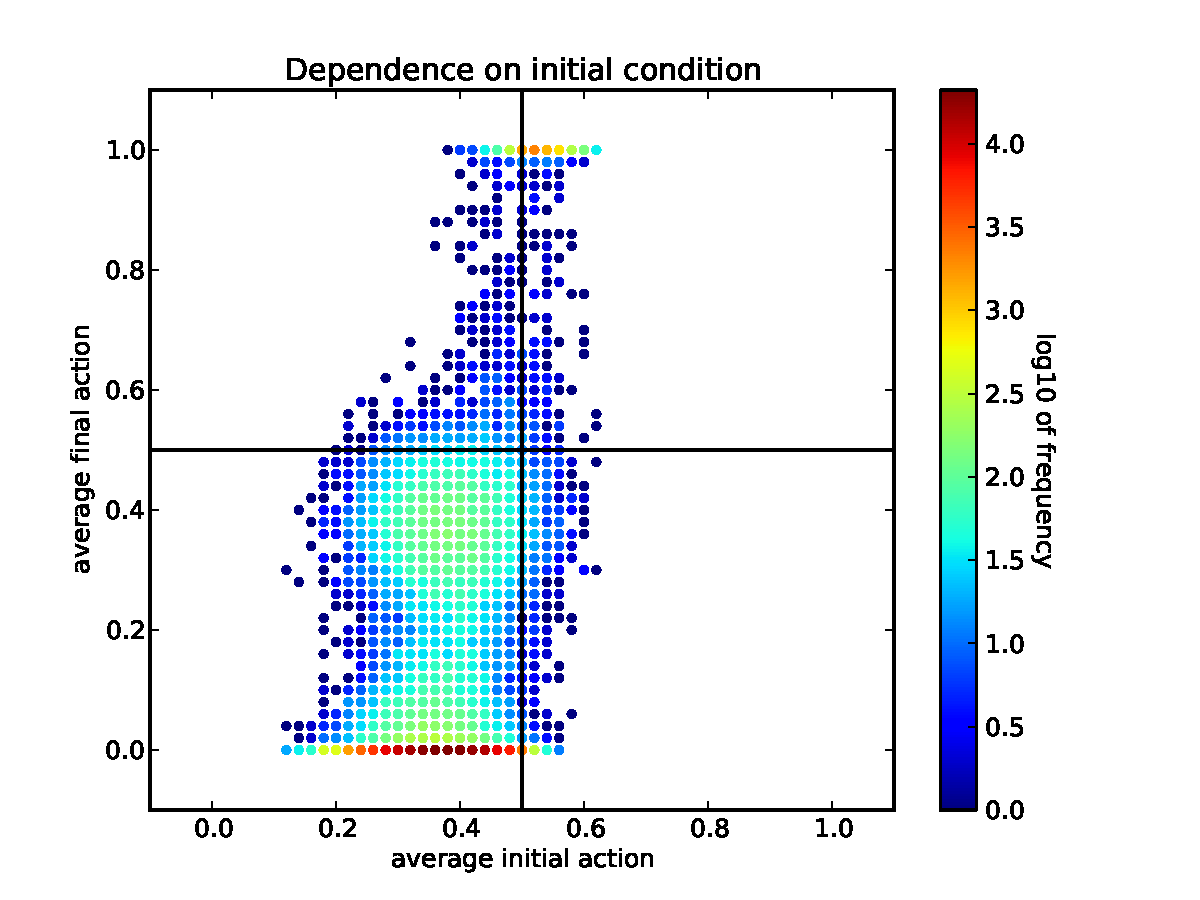
\includegraphics[width=0.5\textwidth]{figures/inf/NEIG_N100_04_SCAT_HIST}
\caption{Case 1 - (I) - neighbor: We plot the average initial action $x_i = \sum_j x_j(0)/N$ vs. the average final action $x_F = \sum_j x_j(T)/N$. Data points are averages over $S$ (1000) simulations and all network densities $\rho$ (20 values equally distributed over the interval $[0,0.95]$. The color code indicates the frequency with which a point occurs in the sample (total size $20 \times 1000$), the scale of the color code is logarithmic of base 10.}
\end{figure}

% =====================================
%
% CASE 1 - (I) - REL NEIGHBOR
%
% =====================================


\begin{figure}[ht]
\centering
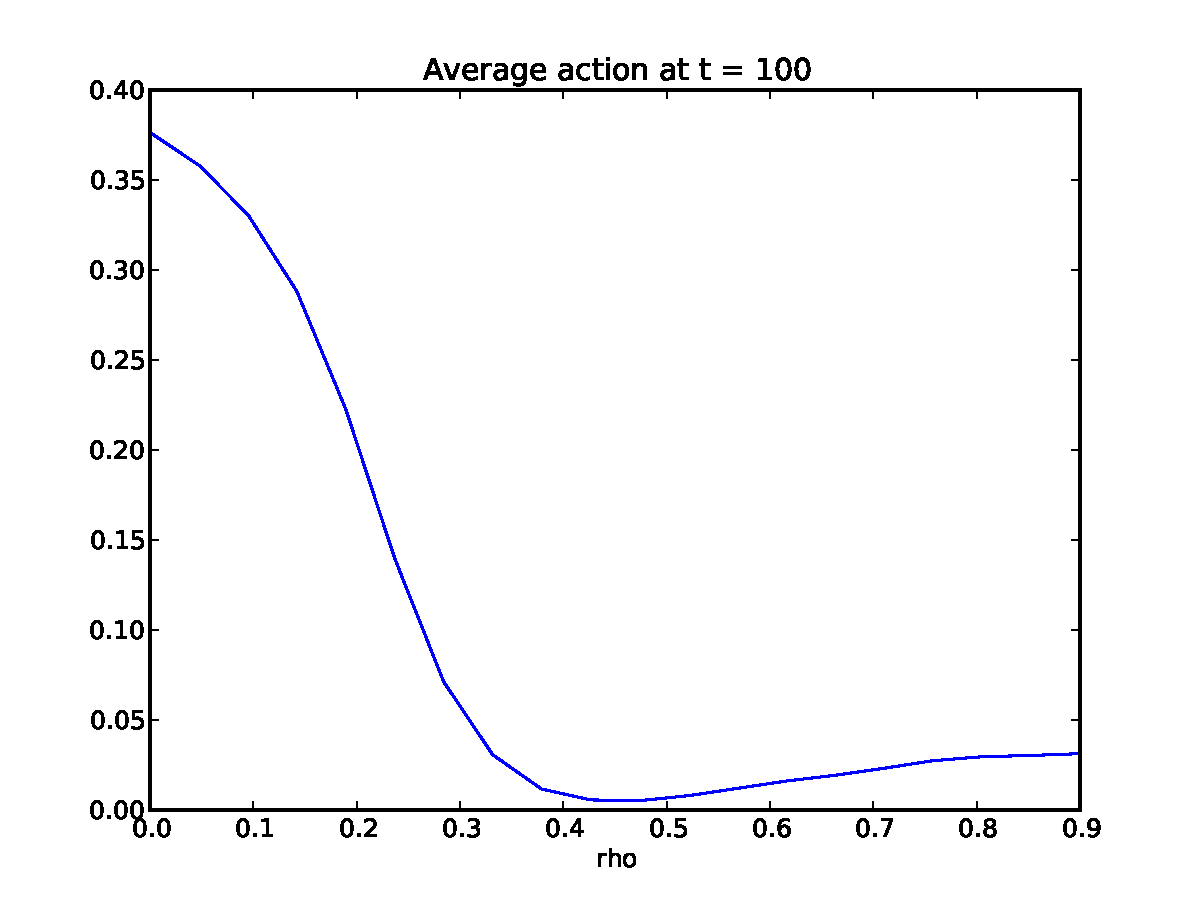
\includegraphics[width=0.5\textwidth]{figures/inf/REL_NEIG_N100_04_AVA}
\caption{Case 1 - (I) - rel neighbor: Average final action of agents as a function of the density of the ER network (rho). The average final action is defined as: $x_F = \sum_j x_j(T)/N$. Data shown is averaged over $S$ (1000) simulations per network density $\rho$. For $\rho = 0$ the agents' actions do not synchronize as they are solely determined by their private belief. As the network density is increased social learning leads to action synchronization.}
\end{figure}

\begin{figure}[ht]
\centering
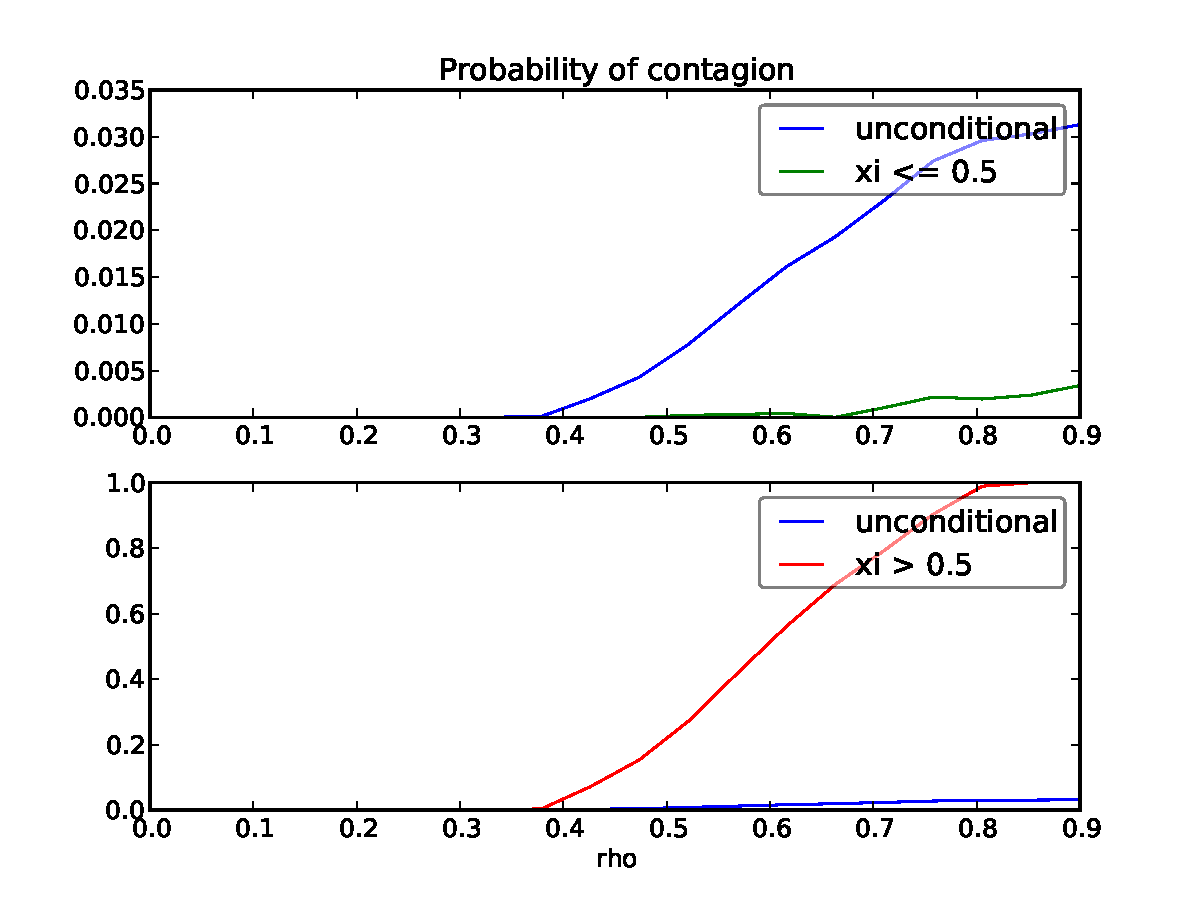
\includegraphics[width=0.5\textwidth]{figures/inf/REL_NEIG_N100_04_CONT}
\caption{Case 1 - (I) - rel neighbor: Fraction of simulations per parameter configuration $S$ (1000) in which agents synchronize on the state non matching action (more than 80\% of agents choose state non-matching action) as a function of network density (rho). We distinguish three cases: (1) unconditional: we compute the fraction based on the full sample $S$. (2) conditional $xi \leq 0.5$: we compute the fraction based on the sub-set of simulations in which the average initial action $x_i = \sum_j x_j(0)/N \leq 0.5$, i.e. when the agents start with a state matching action. (3) conditional $xi > 0.5$: we compute the fraction based on the sub-set of simulations in which the average initial action $x_i = \sum_j x_j(0)/N > 0.5$, i.e. when the agents start with a state non matching action.  }
\end{figure}

\begin{figure}[ht]
\centering
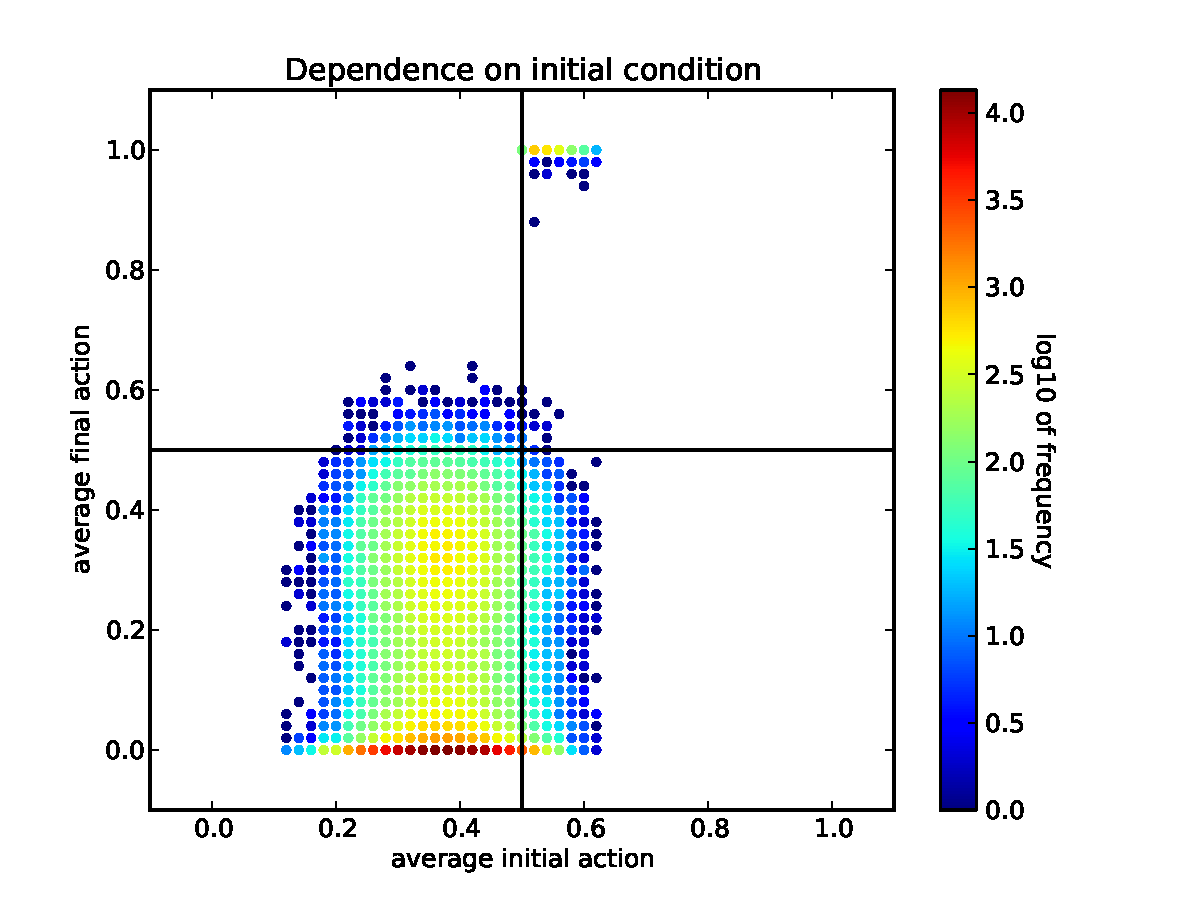
\includegraphics[width=0.5\textwidth]{figures/inf/REL_NEIG_N100_04_SCAT_HIST}
\caption{Case 1 - (I) - rel neighbor: We plot the average initial action $x_i = \sum_j x_j(0)/N$ vs. the average final action $x_F = \sum_j x_j(T)/N$. Data points are averages over $S$ (1000) simulations and all network densities $\rho$ (20 values equally distributed over the interval $[0,0.95]$. The color code indicates the frequency with which a point occurs in the sample (total size $20 \times 1000$), the scale of the color code is logarithmic of base 10.}
\end{figure}

\clearpage

% =====================================
%
% CASE 2 - (U) - EQUAL
%
% =====================================

\begin{figure}[ht]
\centering
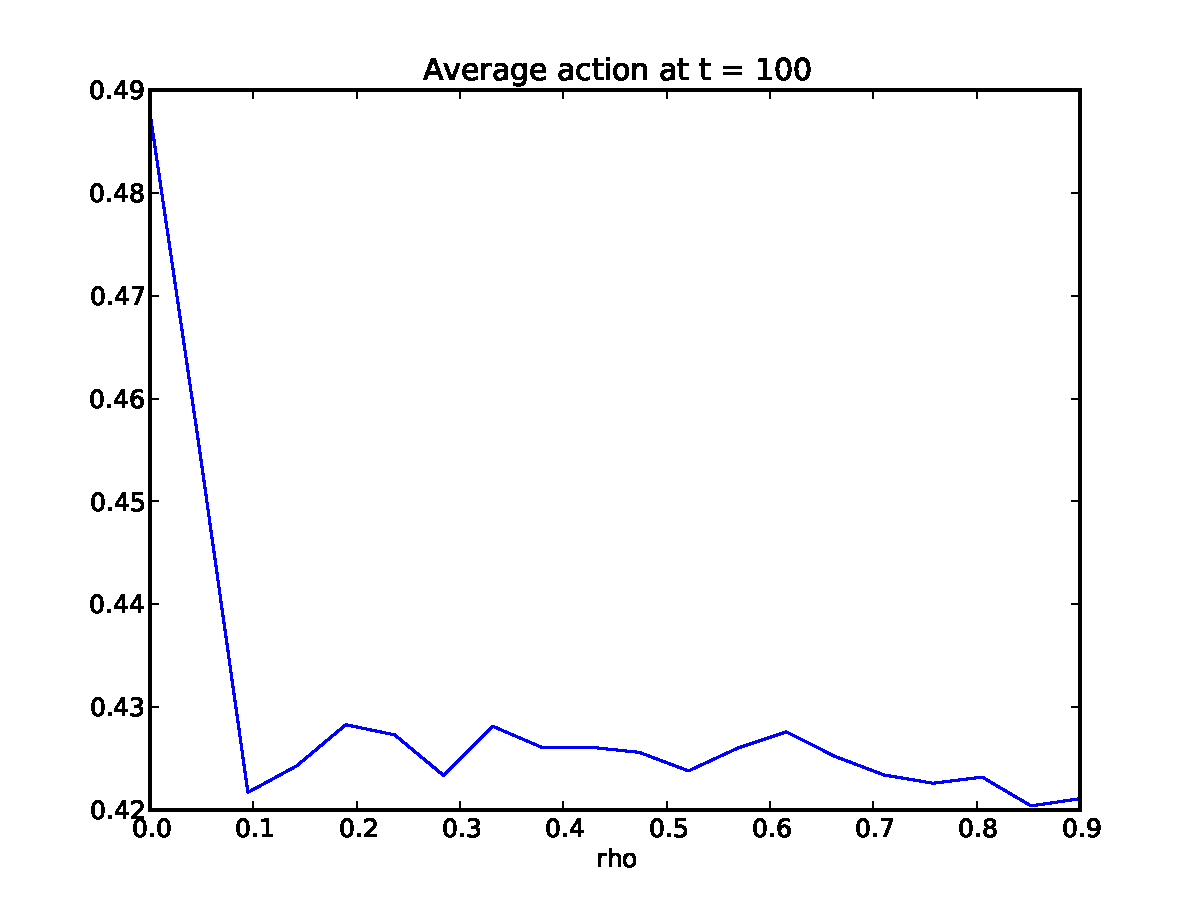
\includegraphics[width=0.5\textwidth]{figures/uninf/EQUAL_N100_049_AVA}
\caption{Case 2 - (U) - equal: Average final action of agents as a function of the density of the ER network (rho). The average final action is defined as: $x_F = \sum_j x_j(T)/N$. Data shown is averaged over $S$ (1000) simulations per network density $\rho$. For $\rho = 0$ the agents' actions do not synchronize as they are solely determined by their private belief. As the network density is increased social learning leads to action synchronization.}
\end{figure}

\begin{figure}[ht]
\centering
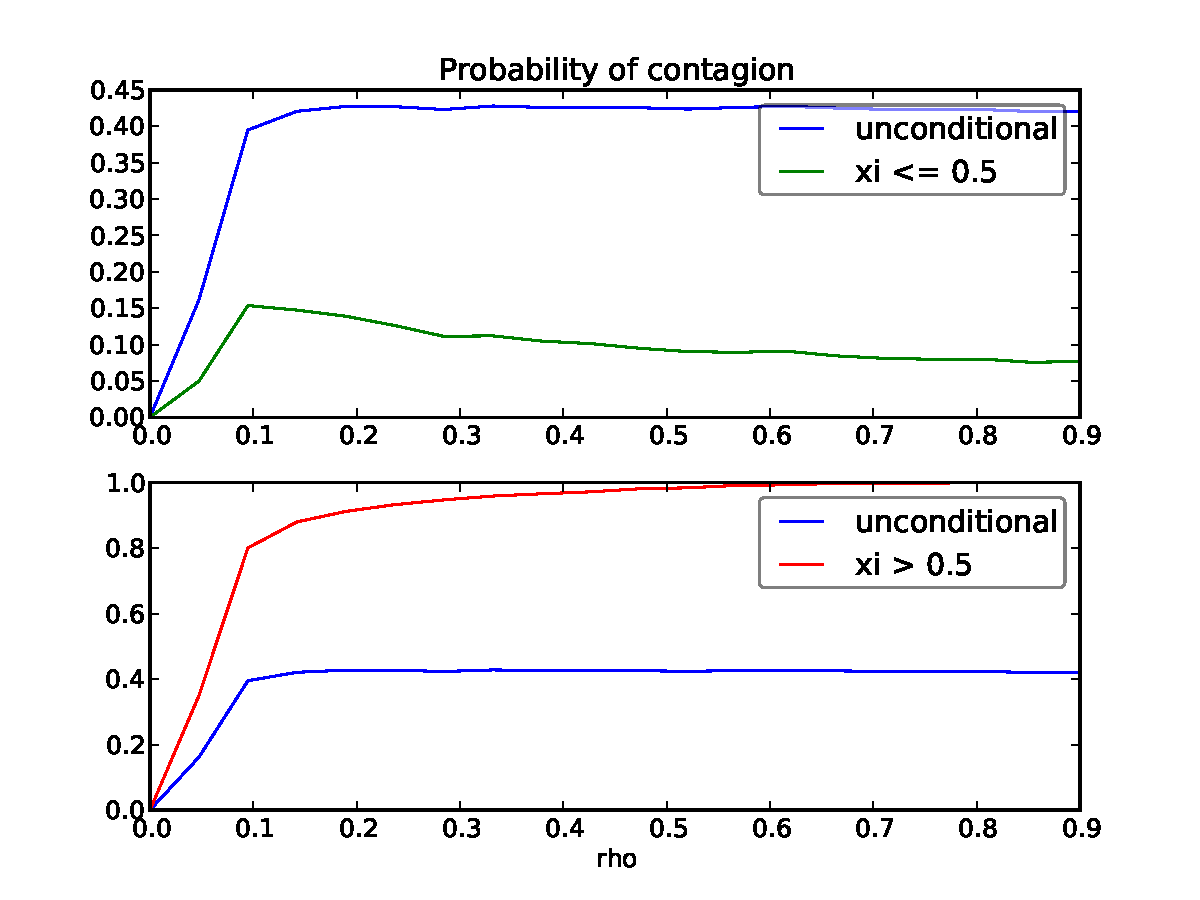
\includegraphics[width=0.5\textwidth]{figures/uninf/EQUAL_N100_049_CONT}
\caption{Case 2 - (U) - equal : Fraction of simulations per parameter configuration $S$ (1000) in which agents synchronize on the state non matching action (more than 80\% of agents choose state non-matching action) as a function of network density (rho). We distinguish three cases: (1) unconditional: we compute the fraction based on the full sample $S$. (2) conditional $xi \leq 0.5$: we compute the fraction based on the sub-set of simulations in which the average initial action $x_i = \sum_j x_j(0)/N \leq 0.5$, i.e. when the agents start with a state matching action. (3) conditional $xi > 0.5$: we compute the fraction based on the sub-set of simulations in which the average initial action $x_i = \sum_j x_j(0)/N > 0.5$, i.e. when the agents start with a state non matching action.  }
\end{figure}

\begin{figure}[ht]
\centering
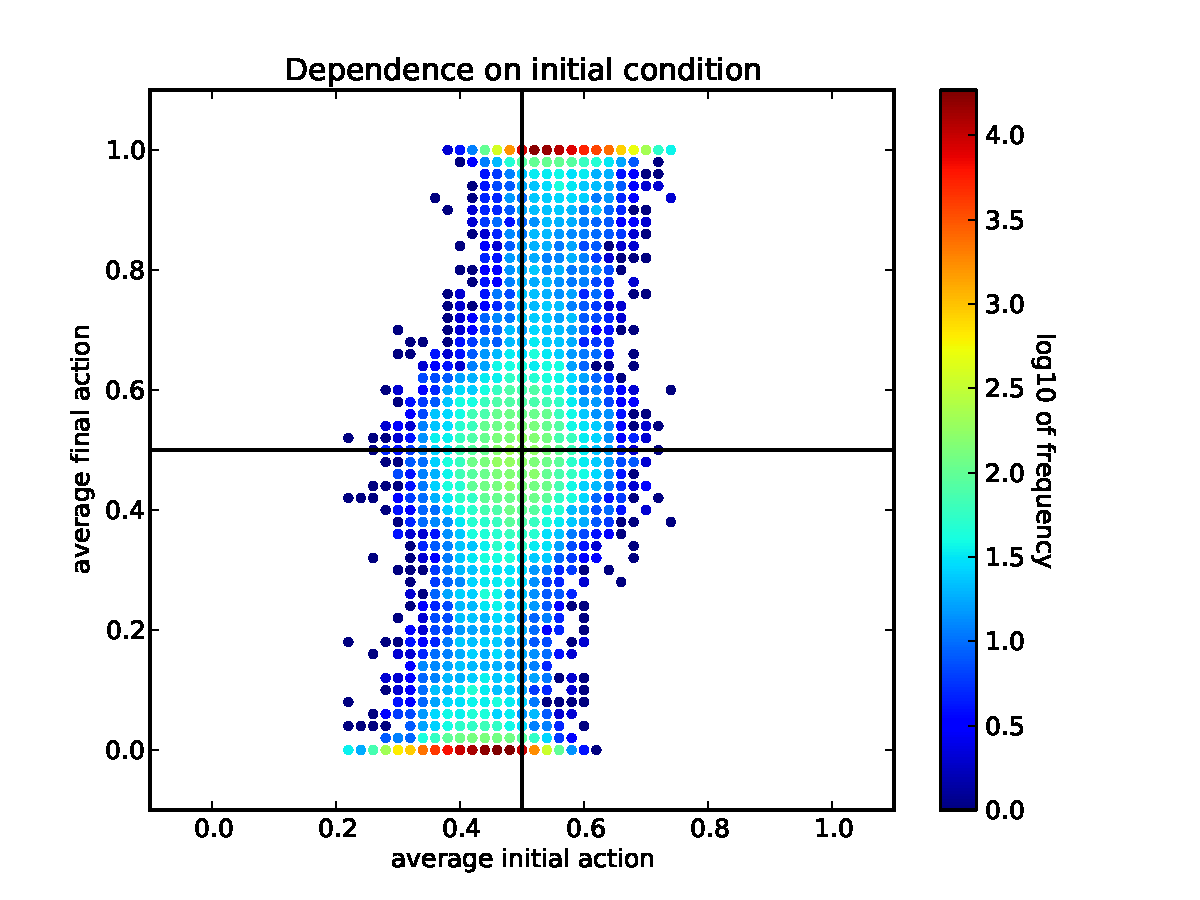
\includegraphics[width=0.5\textwidth]{figures/uninf/EQUAL_N100_049_SCAT_HIST}
\caption{Case 2 - (U) - equal: We plot the average initial action $x_i = \sum_j x_j(0)/N$ vs. the average final action $x_F = \sum_j x_j(T)/N$. Data points are averages over $S$ (1000) simulations and all network densities $\rho$ (20 values equally distributed over the interval $[0,0.95]$. The color code indicates the frequency with which a point occurs in the sample (total size $20 \times 1000$), the scale of the color code is logarithmic of base 10.}
\end{figure}

% =====================================
%
% CASE 2 - (U) - NEIGHBOR
%
% =====================================

\begin{figure}[ht]
\centering
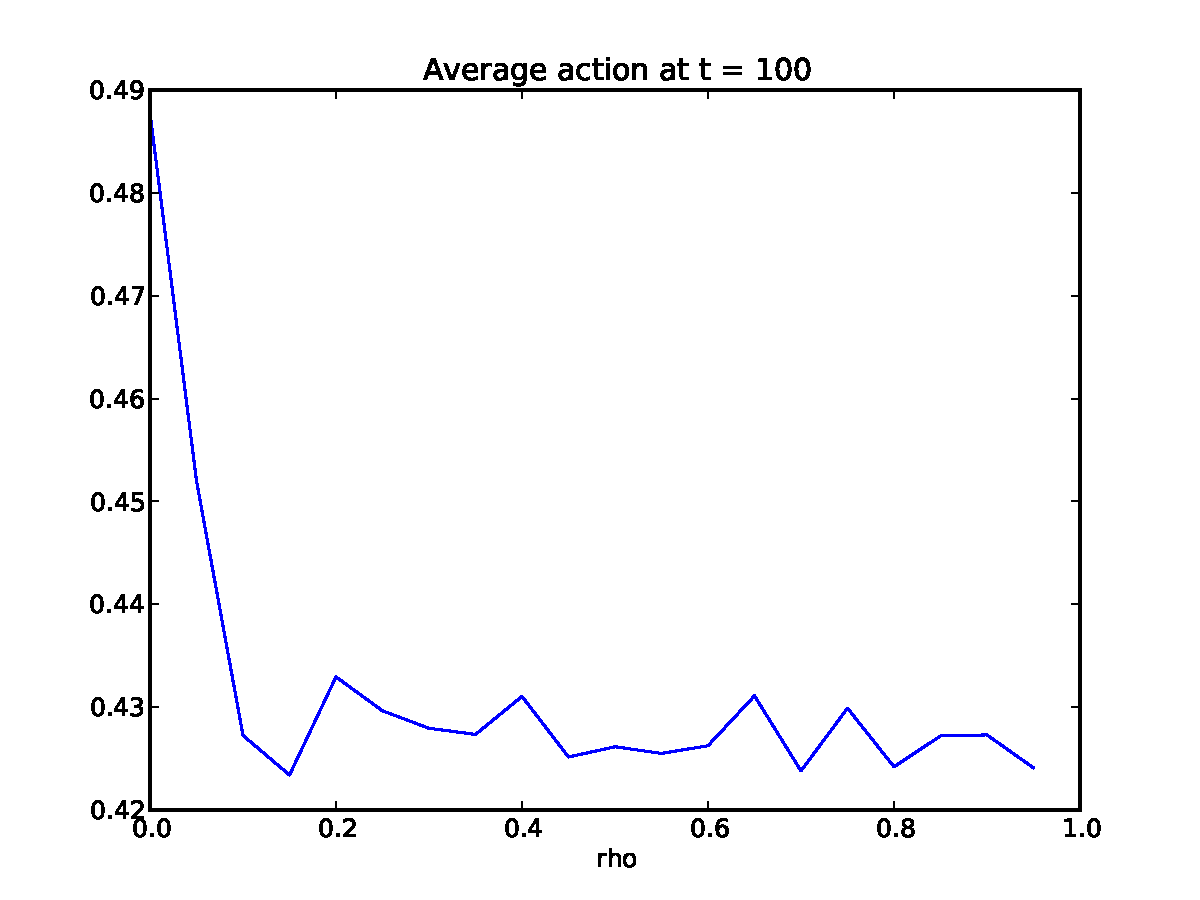
\includegraphics[width=0.5\textwidth]{figures/uninf/NEIG_N100_049_AVA}
\caption{Case 2 - (U) - neighbor: Average final action of agents as a function of the density of the ER network (rho). The average final action is defined as: $x_F = \sum_j x_j(T)/N$. Data shown is averaged over $S$ (1000) simulations per network density $\rho$. For $\rho = 0$ the agents' actions do not synchronize as they are solely determined by their private belief. As the network density is increased social learning leads to action synchronization.}
\end{figure}

\begin{figure}[ht]
\centering
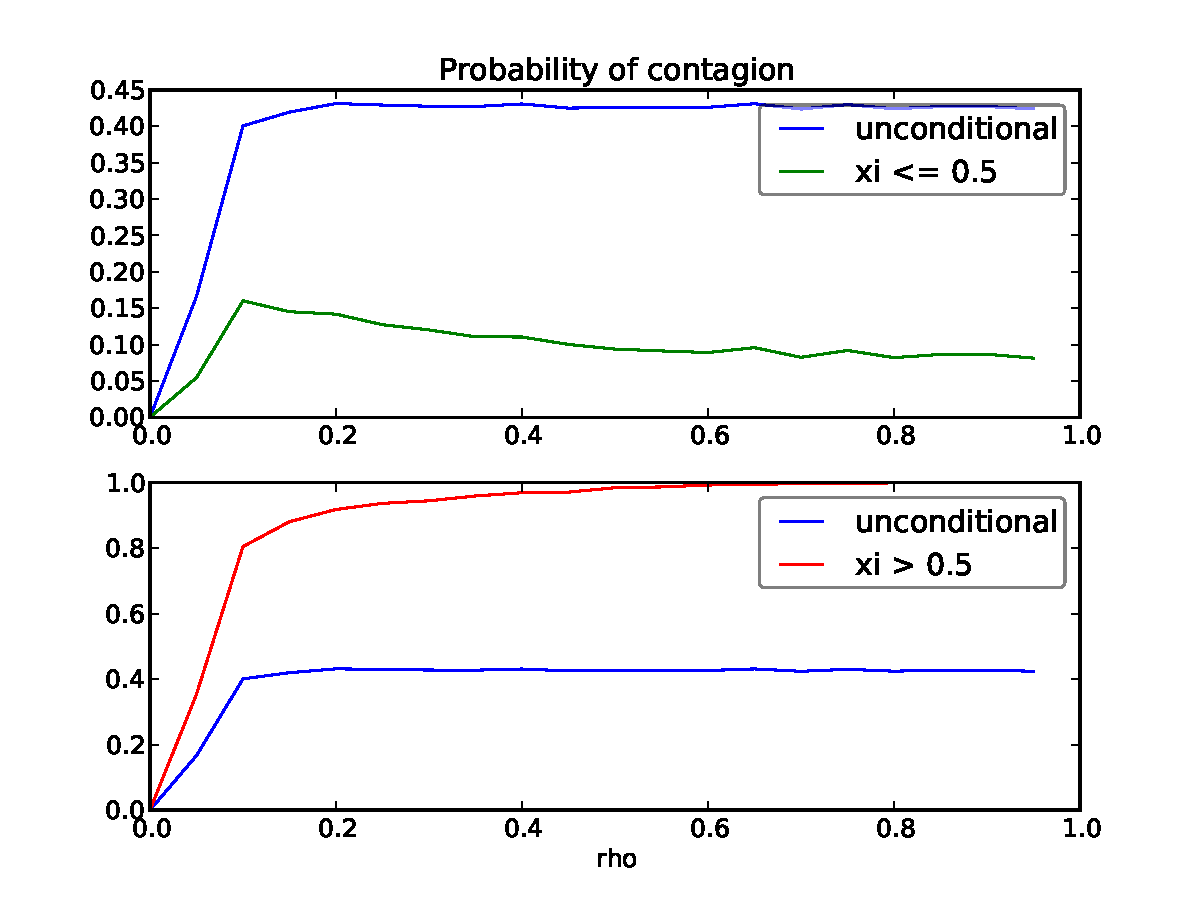
\includegraphics[width=0.5\textwidth]{figures/uninf/NEIG_N100_049_CONT}
\caption{Case 2 - (U) - neighbor: Fraction of simulations per parameter configuration $S$ (1000) in which agents synchronize on the state non matching action (more than 80\% of agents choose state non-matching action) as a function of network density (rho). We distinguish three cases: (1) unconditional: we compute the fraction based on the full sample $S$. (2) conditional $xi \leq 0.5$: we compute the fraction based on the sub-set of simulations in which the average initial action $x_i = \sum_j x_j(0)/N \leq 0.5$, i.e. when the agents start with a state matching action. (3) conditional $xi > 0.5$: we compute the fraction based on the sub-set of simulations in which the average initial action $x_i = \sum_j x_j(0)/N > 0.5$, i.e. when the agents start with a state non matching action.  }
\end{figure}

\begin{figure}[ht]
\centering
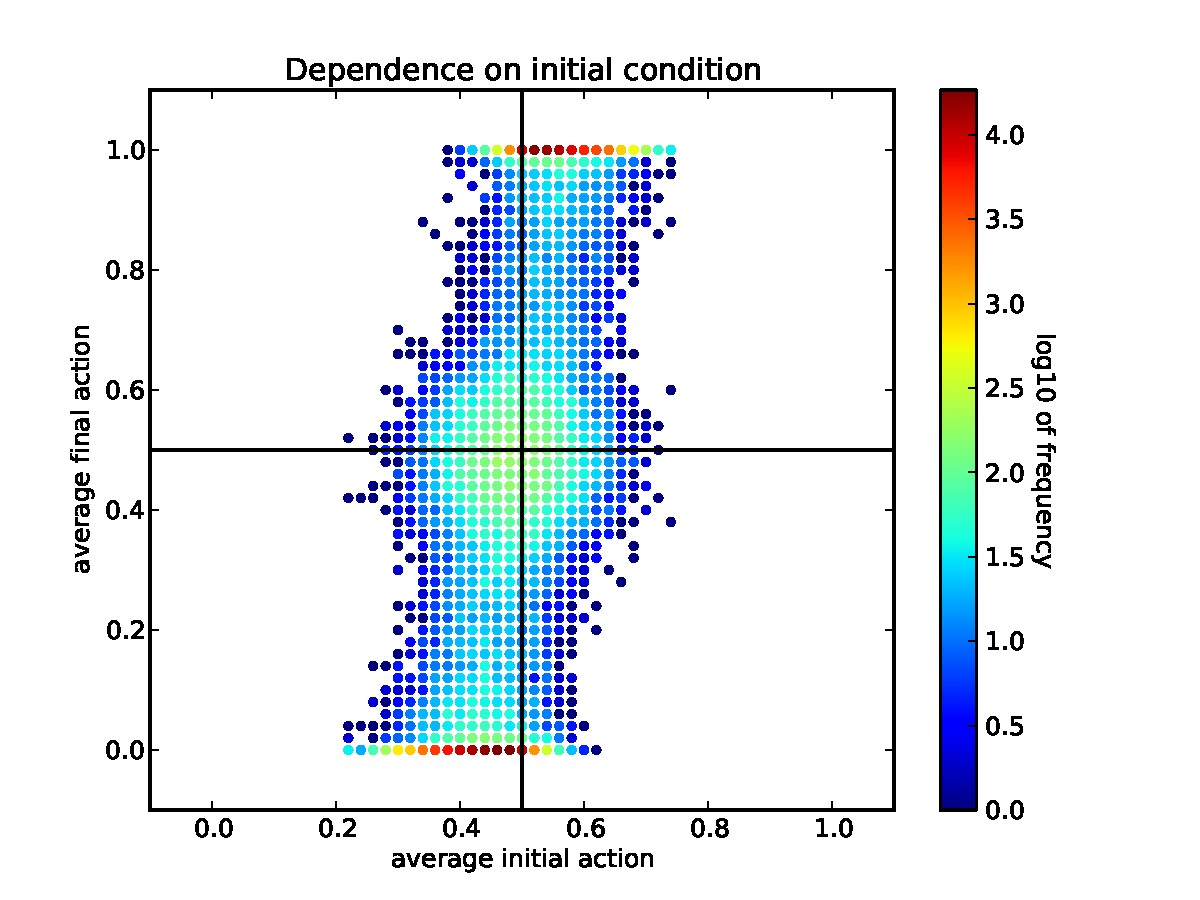
\includegraphics[width=0.5\textwidth]{figures/uninf/NEIG_N100_049_SCAT_HIST}
\caption{Case 2 - (U) - neighbor: We plot the average initial action $x_i = \sum_j x_j(0)/N$ vs. the average final action $x_F = \sum_j x_j(T)/N$. Data points are averages over $S$ (1000) simulations and all network densities $\rho$ (20 values equally distributed over the interval $[0,0.95]$. The color code indicates the frequency with which a point occurs in the sample (total size $20 \times 1000$), the scale of the color code is logarithmic of base 10.}
\end{figure}

% =====================================
%
% CASE 2 - (U) - REL NEIGHBOR
%
% =====================================


\begin{figure}[ht]
\centering
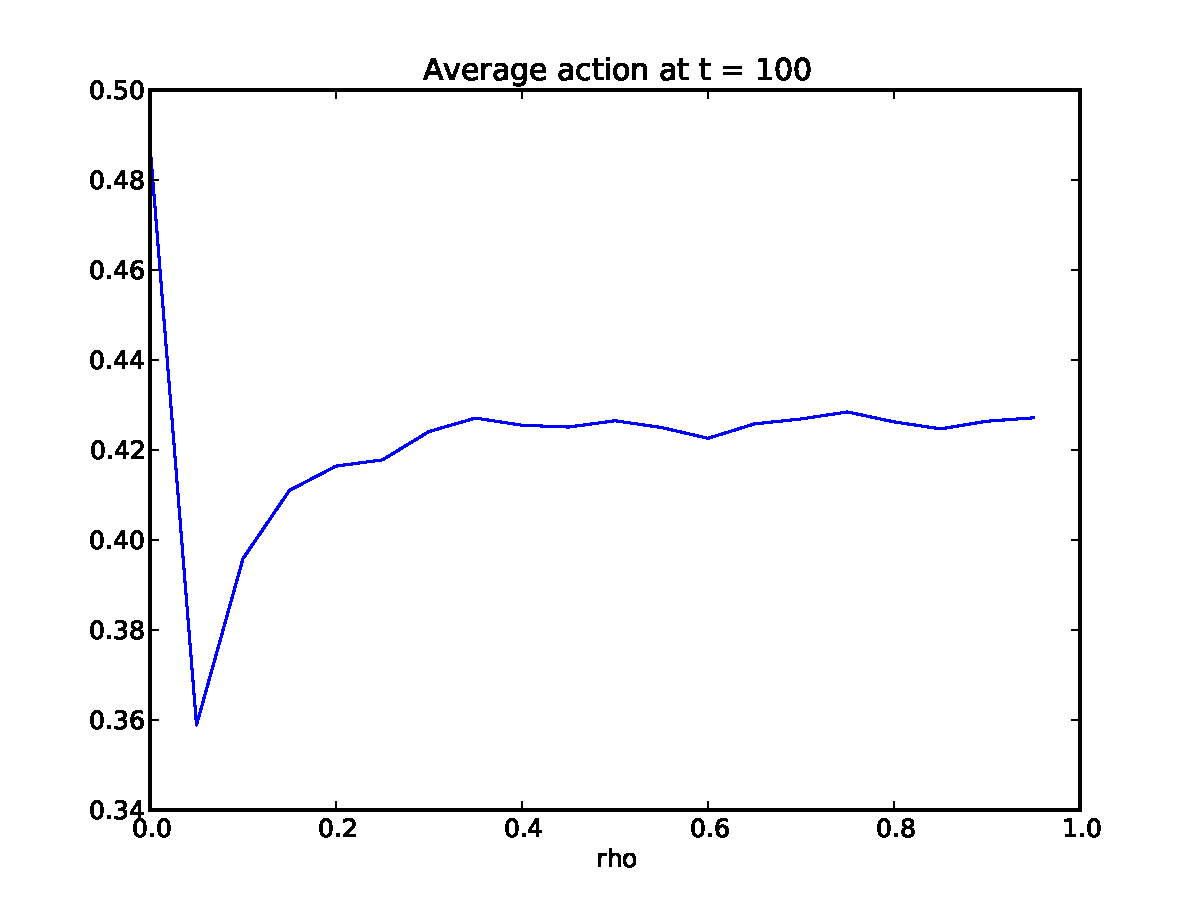
\includegraphics[width=0.5\textwidth]{figures/uninf/REL_NEIG_N100_049_AVA}
\caption{Case 2 - (U) - rel neighbor: Average final action of agents as a function of the density of the ER network (rho). The average final action is defined as: $x_F = \sum_j x_j(T)/N$. Data shown is averaged over $S$ (1000) simulations per network density $\rho$. For $\rho = 0$ the agents' actions do not synchronize as they are solely determined by their private belief. As the network density is increased social learning leads to action synchronization.}
\end{figure}

\begin{figure}[ht]
\centering
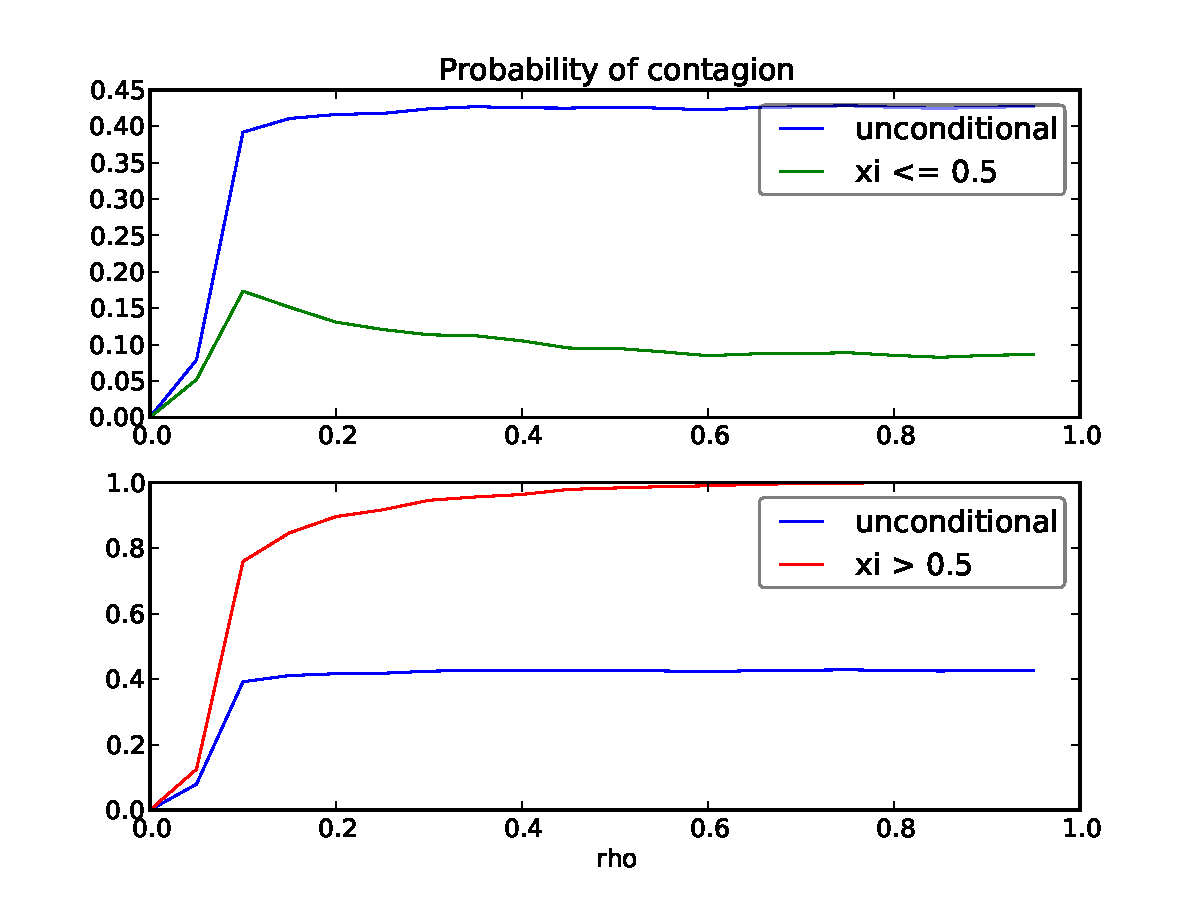
\includegraphics[width=0.5\textwidth]{figures/uninf/REL_NEIG_N100_049_CONT}
\caption{Case 2 - (U) - rel neighbor: Fraction of simulations per parameter configuration $S$ (1000) in which agents synchronize on the state non matching action (more than 80\% of agents choose state non-matching action) as a function of network density (rho). We distinguish three cases: (1) unconditional: we compute the fraction based on the full sample $S$. (2) conditional $xi \leq 0.5$: we compute the fraction based on the sub-set of simulations in which the average initial action $x_i = \sum_j x_j(0)/N \leq 0.5$, i.e. when the agents start with a state matching action. (3) conditional $xi > 0.5$: we compute the fraction based on the sub-set of simulations in which the average initial action $x_i = \sum_j x_j(0)/N > 0.5$, i.e. when the agents start with a state non matching action.  }
\end{figure}

\begin{figure}[ht]
\centering
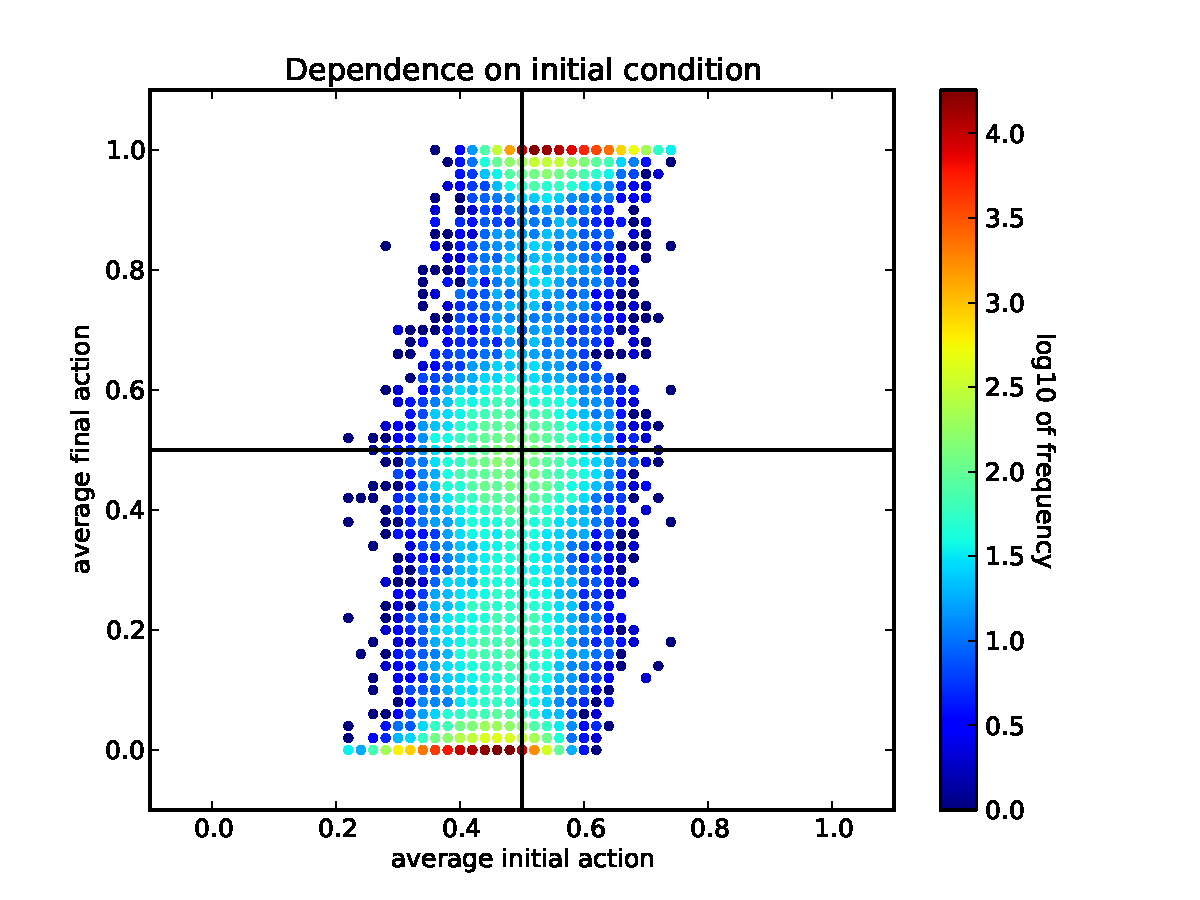
\includegraphics[width=0.5\textwidth]{figures/uninf/REL_NEIG_N100_049_SCAT_HIST}
\caption{Case 2 - (U) - rel neighbor: We plot the average initial action $x_i = \sum_j x_j(0)/N$ vs. the average final action $x_F = \sum_j x_j(T)/N$. Data points are averages over $S$ (1000) simulations and all network densities $\rho$ (20 values equally distributed over the interval $[0,0.95]$. The color code indicates the frequency with which a point occurs in the sample (total size $20 \times 1000$), the scale of the color code is logarithmic of base 10.}
\end{figure}

\clearpage

% =====================================
%
% CASE 3 - (H) - EQUAL
%
% =====================================

\begin{figure}[ht]
\centering
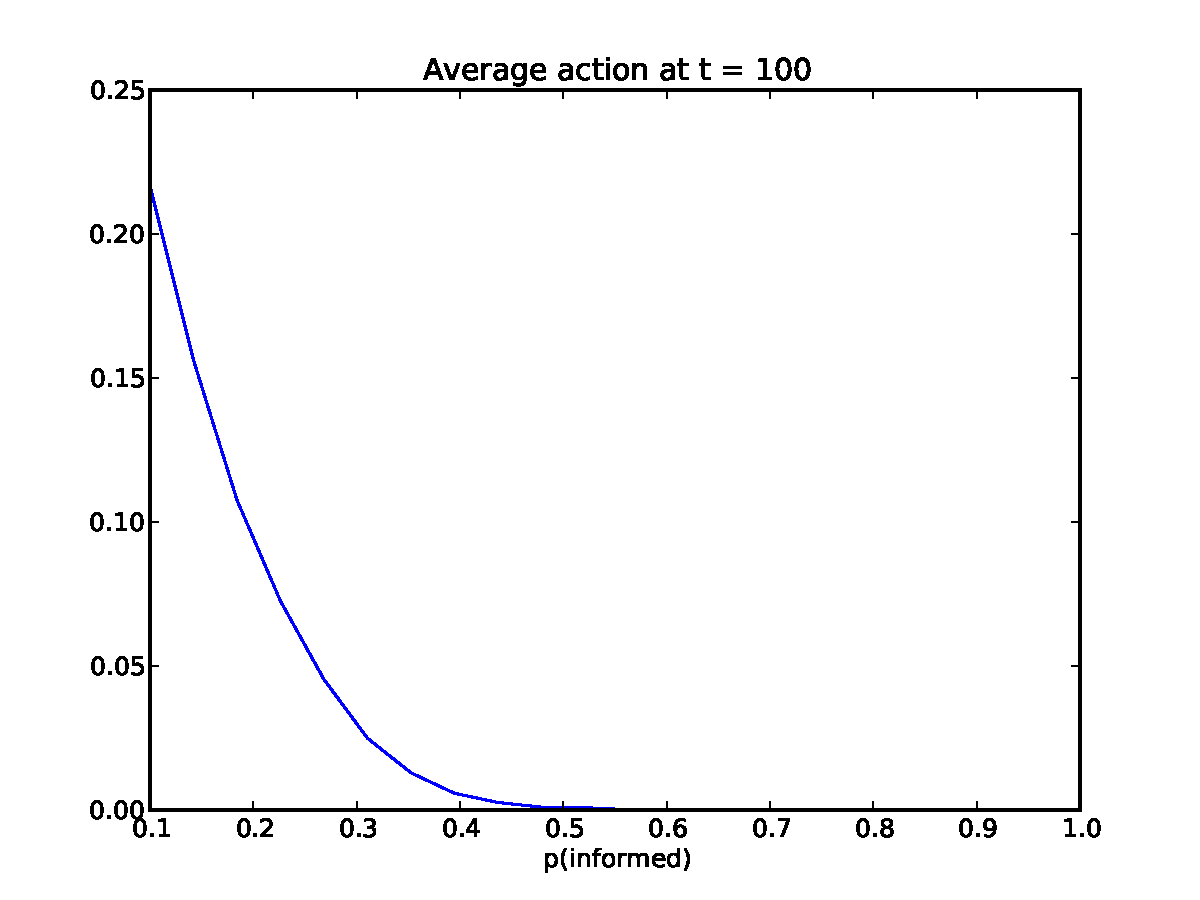
\includegraphics[width=0.5\textwidth]{figures/het/HET_EQUAL_N100_04_AVA}
\caption{Case 3 - (H) - het: Average final action of agents as a function of the probability of being informed $p$. The average final action is defined as: $x_F = \sum_j x_j(T)/N$. Data shown is averaged over $S$ (1000) simulations per probability of being informed $p$.}
\end{figure}

\begin{figure}[ht]
\centering
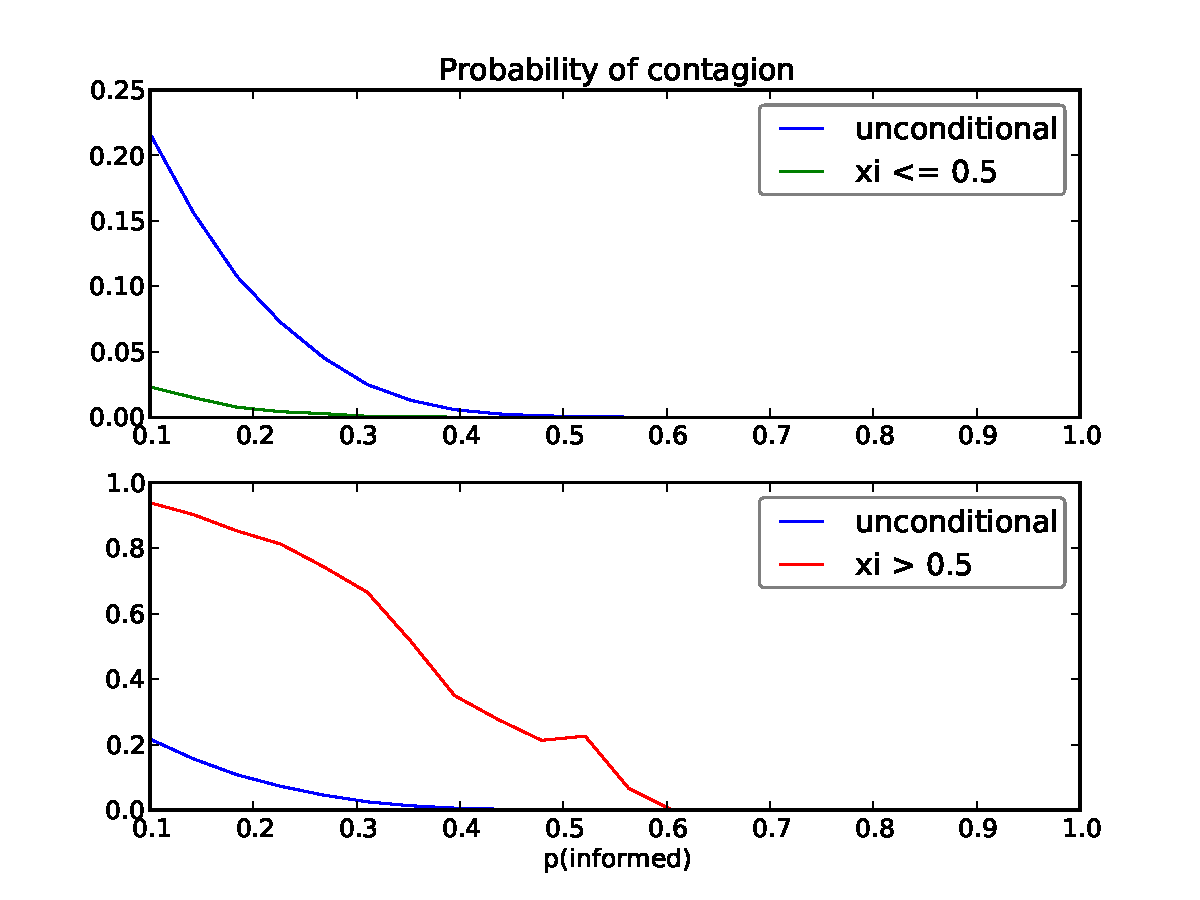
\includegraphics[width=0.5\textwidth]{figures/het/HET_EQUAL_N100_04_CONT}
\caption{Case 3 - (H) - het: Fraction of simulations per parameter configuration $S$ (1000) in which agents synchronize on the state non matching action (more than 80\% of agents choose state non-matching action) as a function of the probability of being informed $p$. We distinguish three cases: (1) unconditional: we compute the fraction based on the full sample $S$. (2) conditional $xi \leq 0.5$: we compute the fraction based on the sub-set of simulations in which the average initial action $x_i = \sum_j x_j(0)/N \leq 0.5$, i.e. when the agents start with a state matching action. (3) conditional $xi > 0.5$: we compute the fraction based on the sub-set of simulations in which the average initial action $x_i = \sum_j x_j(0)/N > 0.5$, i.e. when the agents start with a state non matching action.  }
\end{figure}

\end{document}